\chapter{Kết quả thực nghiệm và đánh giá}
\label{chap:results}

\section{Thiết kế kiểm chứng và phép đo}

Thực nghiệm sử dụng dữ liệu sinh có kiểm soát, gồm đường đi, chuỗi hình thoi, cactus, partial $k$-tree và ladder. Các họ đồ thị làm thay đổi riêng chiều dài, số nhãn, mật độ nhãn hoặc độ rộng, nhằm phân biệt yếu tố cấu trúc với kích thước danh sách cạnh thời gian. Cả hai ngữ nghĩa thời gian được kiểm tra; các ví dụ tăng tốc dưới đây gắn với từng họ dữ liệu cụ thể, không được suy rộng thành tăng tốc trên mọi đồ thị.

Bộ kiểm chứng gồm vét cạn các đồ thị thời gian nhỏ, dữ liệu ngẫu nhiên, biến đổi bảo toàn đáp án và Graph Atlas. Phạm vi vét cạn là $n\le4,r\le2$ và $n=5,r=1$; chưa vét cạn $n=5,r=2$. Graph Atlas cung cấp $1\,253$ đồ thị không đẳng cấu đến bảy đỉnh~\cite{atlas}; đề tài chọn $495$ đồ thị với $n\ge2$ và treewidth không quá hai, thử mọi cặp đầu cuối có thứ tự, ba cách gán nhãn và hai ngữ nghĩa.

Đối chứng tính đúng dùng bộ liệt kê trực tiếp cạnh thời gian, công thức đóng trên các họ có cấu trúc và bộ đếm độc lập. Các số đếm đều dùng số nguyên không giới hạn 64 bit. Với đường dài $P$ mà mọi cạnh hoạt động ở mọi hạng, hai đáp án là
\[
  C_{\le}=\binom{r+P-1}{P},\qquad C_{<}=\binom{r}{P}.
\]
Chuỗi $k$ hình thoi có $2^k$ tuyến, mỗi tuyến dài $2k$, nên nhân các công thức tương ứng với $2^k$. Các công thức này kiểm tra cả trường hợp đáp án lớn và trường hợp nghiêm ngặt trả về $0$ vì không đủ nhãn.

\begin{table}[htbp]{Phạm vi kiểm chứng tính đúng của các thuật toán.}
\label{tab:audit}
\centering\small
\setlength{\tabcolsep}{4pt}
\renewcommand{\arraystretch}{1.16}
\begin{tabular}{p{5.2cm}rrr}
\toprule
Chiến dịch & \shortstack{Lượt truy vấn/\\ngữ nghĩa} & Đối chiếu & Sai lệch \\
\midrule
Vét cạn nhỏ & 140\,048 & 491\,664 & 0 \\
Ngẫu nhiên và biến đổi & 8\,400 & 26\,800 & 0 \\
Graph Atlas, $w\le2$ & 111\,408 & 222\,816 & 0 \\
\textbf{Tổng lượt} & 259\,856 & 741\,280 & 0 \\
\bottomrule
\end{tabular}
\par\vspace{3pt}\begin{minipage}{0.97\linewidth}\footnotesize Một lượt truy vấn/ngữ nghĩa có thể tạo nhiều đối chiếu giữa các thuật toán. Các tổng trên không phải số đồ thị khác nhau.\end{minipage}
\end{table}


Tổng cộng có \QueryModeCases{} lượt truy vấn/ngữ nghĩa và \AuditComparisons{} lượt đối chiếu, không có sai lệch. Kết quả này là bằng chứng thực nghiệm về tính đúng trong phạm vi thử, không thay thế lập luận ở Chương~\ref{chap:algorithms}. Một số bộ đối chứng chia sẻ thủ tục phụ; vì vậy số lượt đối chiếu cũng không được diễn giải thành từng ấy phép xác nhận hoàn toàn độc lập.

Bộ benchmark gồm \BenchmarkCases{} trường hợp và \RawRows{} bản ghi, trong đó có \CompletedSolverCases{} trường hợp thuật toán hoàn thành đủ bảy mẫu. Mỗi cấu hình có một bước chạy làm nóng/hiệu chỉnh, rồi bảy mẫu trong các tiến trình riêng; mỗi mẫu có thể lặp nội bộ để nhắm thời lượng khoảng $10$ ms. Thứ tự thuật toán được xáo trộn, giới hạn tiến trình là $3$ giây và không gian địa chỉ là $1\,536$ MiB. Có $15$ lượt hết giờ và $3$ lượt bỏ qua vì ngân sách; chúng được ghi nhận, không thay bằng số đo giả và không đưa vào tỷ số ghép cặp.

Môi trường đo là Intel Core i9-9980HK, RAM khoảng $15$ GiB, Linux 6.12.93 và GCC 14.3.0, tối ưu hóa \texttt{-O3}. Tiến trình được ghim vào một CPU nhưng tần số CPU không cố định. Thời gian thuật toán bao gồm việc đọc/xác thực phân rã bổ trợ, không bao gồm đọc đồ thị thời gian và sinh phân rã. Bộ nhớ là đỉnh RSS sau khi tiến trình bắt đầu chương trình mới, tính theo MiB. Các điều kiện này giới hạn khả năng so sánh trực tiếp với số đo trên máy khác.

\section{Tăng tốc và ý nghĩa của đối chứng}

Với trường hợp ghép cặp $i$, đặt $q_i=T_{\mathrm{base},i}/T_{\mathrm{new},i}$, trong đó $T_{\mathrm{base},i}$ và $T_{\mathrm{new},i}$ lần lượt là trung vị thời gian đối chứng và đề xuất qua bảy mẫu. Đề tài dùng trung bình nhân
\[
  \operatorname{GM}=\exp\left(\frac{1}{K}\sum_{i=1}^{K}\log q_i\right),
\]
để tổng hợp các tỷ số trên $K$ trường hợp hoàn thành ở cả hai phía. GM không phải tỷ số của hai tổng thời gian và không bao gồm các trường hợp hết giờ.

\begin{table}[htbp]{Tăng tốc trên các trường hợp ghép cặp hoàn thành.}
\label{tab:speedups}
\centering\small
\setlength{\tabcolsep}{4pt}
\renewcommand{\arraystretch}{1.16}
\begin{tabular}{p{2.4cm}p{3.1cm}p{2.6cm}rr}
\toprule
Họ đồ thị & Đối chứng & Đề xuất & $K$ & GM \\
\midrule
Rừng dày & Truy hồi bài gốc & Tổng tiền tố & 47 & \num{16.1} \\
TTSP dày & Ma trận nội bộ & Quét sự kiện & 45 & \num{5.24} \\
Partial 2-tree & DP nội bộ cũ & DP tối giản & 24 & \num{3.8} \\
Cactus & DP tổng quát & Quét theo block & 8 & \num{78.9} \\
\bottomrule
\end{tabular}
\par\vspace{3pt}\begin{minipage}{0.97\linewidth}\footnotesize GM là trung bình nhân của tỷ số thời gian đối chứng/đề xuất; $K$ là số trường hợp ghép cặp. Chỉ đối chứng ở hàng rừng tái hiện truy hồi của bài báo gốc; các hàng còn lại là đối chứng của dự án.\end{minipage}
\end{table}


Trên rừng dày, tổng tiền tố nhanh hơn truy hồi trực tiếp với GM \ForestGM{} lần. Hình~\ref{fig:forest} cho thấy độ chênh tăng khi số nhãn tăng trên một đường dài cố định, phù hợp với việc bỏ một vòng tính tổng theo $r$. Tuy nhiên, bản quét nhãn thưa không luôn nhanh nhất trên dữ liệu dày. Khi giữ $P=r=1\,000$ nhưng mỗi cạnh chỉ có một nhãn, bản thưa nhanh hơn bản dày khoảng \SparseControlSpeed{} lần; lựa chọn biểu diễn cần phụ thuộc mật độ.

\begin{figure}[htbp]{Thời gian trên đường dài $1\,000$ cạnh theo số hạng $r$; hai trục dùng thang lô-ga-rít, đơn vị thời gian là ms. Mỗi điểm là trung vị, thanh sai số biểu diễn tứ phân vị $Q_1$--$Q_3$. Ba đường là truy hồi bài gốc được tái hiện, tổng tiền tố dày và quét nhãn thưa. Điểm hết giờ không được vẽ thành số đo.}
\label{fig:forest}
\centering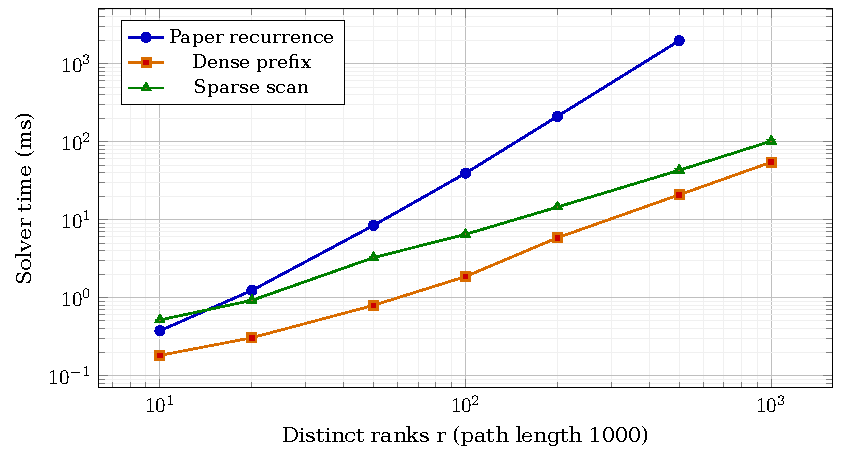
\includegraphics[width=0.94\linewidth]{../results/figures/forest-scaling.pdf}
\end{figure}

Trên TTSP dày, quét sự kiện đạt GM \TTSPGM{} lần so với ma trận truyền nội bộ. Với $k=256$, $r=32$, dữ liệu có $1\,024$ cạnh nền và $32\,768$ cạnh thời gian; trung vị giảm từ \TTSPMatrixTime{} ms xuống \TTSPEventsTime{} ms, tương đương \TTSPExampleSpeed{} lần. Đỉnh RSS lớn nhất qua bảy mẫu giảm từ \TTSPMatrixRSS{} xuống \TTSPEventsRSS{} MiB; đáp án dài $424$ bit. Đây là cải thiện cả thời gian và bộ nhớ trên cùng một bài toán, không phải kết quả tính theo mô-đun.

Một trường hợp bổ sung $k=32,r=128$ đạt tỷ số \TTSPExtraSpeed{} lần, nhưng không được dùng thay cho GM của họ TTSP dày. Trên trường hợp thưa có $r=\TTSPSparseRanks$, thuật toán sự kiện hoàn thành trong \TTSPSparseTime{} ms, còn ma trận bị bỏ qua theo giới hạn ngân sách. Vì không có số đo ma trận, báo cáo không suy ra tỷ số tăng tốc cho trường hợp này.

Trên cactus, quét tuyến khối đạt GM \CactusGM{} lần so với DP tổng quát; so sánh phản ánh lợi ích của thuật toán chuyên biệt khi nhận diện đúng cấu trúc. Trên partial 2-tree, DP tối giản đạt GM \PartialGM{} lần so với DP nội bộ cũ. Chỉ hàng rừng ở Bảng~\ref{tab:speedups} đối chiếu với truy hồi của bài báo gốc; các hàng khác không phải phép đo trực tiếp mã nguồn hoặc thời gian do tác giả bài báo công bố.

\section{Đóng góp của tối ưu và trường hợp khó}

Thực nghiệm loại bỏ từng tối ưu ở Bảng~\ref{tab:ablation} giúp giải thích nguồn cải thiện của DP. Xóa nhãn đầu cuối làm giảm số trạng thái tạo; bỏ đồng thời cắt tỉa và xóa nhãn đưa số trạng thái trở lại gần bản cũ. Giữ mọi bảng con làm tăng số trạng thái đồng thời sống nhưng không làm tăng số trạng thái phải tạo. Như vậy, giảm không gian trạng thái và giảm thời gian giữ bảng là hai tác động khác nhau, không nên đồng nhất với một chỉ số bộ nhớ duy nhất.

\begin{table}[htbp]{Đóng góp của từng tối ưu trên ba partial 2-tree ($n=24$, $r=8$).}
\label{tab:ablation}
\centering\small
\setlength{\tabcolsep}{4pt}
\renewcommand{\arraystretch}{1.16}
\begin{tabular}{p{6cm}rrr}
\toprule
Cấu hình & Thời gian (ms) & Trạng thái tạo & \shortstack{Trạng thái\\sống cực đại} \\
\midrule
DP nội bộ cũ & \num{32.4} & 18\,785 & 18\,785 \\
DP đầy đủ & \num{5.46} & 6\,801 & 854 \\
Không xóa nhãn đầu cuối & \num{11.8} & 11\,324 & 2\,197 \\
Không cắt tỉa và xóa nhãn & \num{24.9} & 18\,785 & 4\,957 \\
Không lọc cặp ghép & \num{6.49} & 6\,801 & 854 \\
Giữ mọi bảng con & \num{5.73} & 6\,801 & 6\,801 \\
\bottomrule
\end{tabular}
\par\vspace{3pt}\begin{minipage}{0.97\linewidth}\footnotesize Thời gian là trung bình nhân của ba trung vị; hai cột cuối là trung vị theo trường hợp. Số trạng thái sống là số trạng thái đồng thời đang được giữ, không phải số đỉnh đồ thị.\end{minipage}
\end{table}


Khi bỏ cắt tỉa, phép xóa nhãn đầu cuối cũng phải tắt vì điều kiện đúng của phép xóa phụ thuộc bậc được phép tại $s,z$. Hàng đó không đo riêng tác động của cắt tỉa. Thực nghiệm loại bỏ từng tối ưu chỉ dùng ba trường hợp; kết quả hỗ trợ cơ chế thuật toán, chưa đủ để khẳng định hiệu ứng giống nhau trên mọi phân bố đầu vào.

Đồ thị ladder kiểm tra miền rộng hơn cactus và truy vấn hai cực TTSP có sẵn. Với $c$ cột, truy vấn từ góc trên-trái đến góc dưới-phải có $2^{c-1}$ đường đi tĩnh. Bảng~\ref{tab:ladder} cho thấy thuật toán liệt kê bắt đầu hết giờ ở kích thước lớn, trong khi DP mới vẫn đếm chính xác ở $c=64$, nơi có $2^{63}$ tuyến tĩnh. Đây là bằng chứng cho khả năng tổng hợp nhiều nghiệm, không chỉ cải thiện hằng số trên số lượng đường đi nhỏ.

\begin{table}[htbp]{Ladder có độ rộng hai, $r=4$, đầu cuối trên-trái và dưới-phải.}
\label{tab:ladder}
\centering\small
\setlength{\tabcolsep}{4pt}
\renewcommand{\arraystretch}{1.16}
\begin{tabular}{lrrrr}
\toprule
Số cột $c$ & Đường đi tĩnh & Liệt kê (ms) & DP cũ (ms) & DP mới (ms) \\
\midrule
8 & $2^{7}$ & \num{0.25} & \num{3.73} & \num{0.876} \\
16 & $2^{15}$ & \num{138} & \num{9.07} & \num{2.04} \\
24 & $2^{23}$ & Hết giờ & \num{14.2} & \num{3.16} \\
64 & $2^{63}$ & Hết giờ & \num{40.6} & \num{9.38} \\
\bottomrule
\end{tabular}
\par\vspace{3pt}\begin{minipage}{0.97\linewidth}\footnotesize Mỗi số đo là trung vị của bảy mẫu. Hết giờ nghĩa là tiến trình không hoàn thành trong 3 giây; không thay bằng một thời gian giả để tính tỷ số tăng tốc.\end{minipage}
\end{table}


Các hạn chế còn lại gồm dữ liệu chủ yếu là dữ liệu sinh, số hạt giống ở một số phép đo ít và tần số CPU chưa cố định. Khi $w$ hoặc $r$ tăng, số trạng thái của DP vẫn có thể lớn. Do đó, kết quả hiện tại hỗ trợ đóng góp về thuật toán có cấu trúc và thực nghiệm tái lập, nhưng chưa xác lập ưu thế trên mọi mạng thực tế hoặc tính mới toàn diện so với toàn bộ văn liệu hiện hành.
